\documentclass[12pt,a4paper]{report}
\usepackage{amsmath, amssymb, amsthm}
\usepackage{enumitem}
\usepackage{hyperref}
\usepackage{bm}
\usepackage[utf8]{inputenc}     % if you need it
\usepackage[T1]{fontenc}        % if you need it
% \usepackage{subcaption}         % defines the subfigure environment
\usepackage{grffile}
\usepackage{placeins}    
\usepackage[a4paper,margin=1in]{geometry}
\usepackage{graphicx}
\usepackage{subcaption}
\usepackage{booktabs}
\usepackage{float}       % for [H]
\usepackage{placeins}    % for \FloatBarrier

\hypersetup{
    colorlinks=true,
    linkcolor=blue,
    urlcolor=blue,
    citecolor=blue
}

\title{Lab Notes: Thermo-couple Experiment}
\author{Elie-Peter Habib}
\date{\today}

\begin{document}
%--------------------------
\maketitle

\tableofcontents
\pagebreak
%--------------------------

%================================
%==========CHAPTER 1
%================================
\chapter{First part}


\section{theoretical background}

The thermoelectric phenomenon was discovered by Thomas Johann Seebeck in the early 1820s. Seebeck observed that when two different metals are joined together at two junctions, forming a closed loop, and these junctions are maintained at different temperatures, an electric current flows through the circuit. Initially, Seebeck mistakenly attributed this effect to magnetic polarization of the metals, but later it was correctly understood as an electromotive force (voltage) generated due to the temperature difference.
\\

This voltage arises due to thermoelectric properties which depend on the interactions between heat flow and the behavior of electric charge carriers in metals. The phenomenon is broadly categorized under thermoelectric effects, with the Seebeck effect being one of the three primary effects:

\begin{enumerate}
    \item \textbf{Seebeck Effect}: Generation of a voltage when there is a temperature difference across the junctions of two different metals.
    \item \textbf{Peltier Effect}: Heat absorption or release at the junction of two different metals when an electric current flows through the junction.
    \item \textbf{Thomson Effect}: Heat absorption or release when current flows through a conductor subjected to a temperature gradient.
\end{enumerate}

A typical thermocouple consists of two dissimilar metals joined at both ends. When the junctions are at different temperatures ($T_1$ and $T_2$), a voltage ($V$) is generated, which can be measured. Importantly, a thermocouple measures the temperature difference, not absolute temperature. In order to measure the abolute tempreture one junction, called the reference junction, is maintained at a known temperature, and the other junction measures the unknown temperature.

The voltage generated in the thermocouple is a function of the types of metal (spicifically thier band gap), call them A and B, and  the reference tempreture and the unkown tempreture. Although the first three are known so the voltage is actually a function of the unknown temperature.

\paragraph{}
As with every other function, the relation between the voltage and the temperature difference $V(\Delta T)$ can be approximated by a Taylor polynomial expansion:
\begin{equation}
    V(\Delta T) = C_0 + C_1 \Delta T + C_2 (\Delta T)^2 + \ldots
\end{equation}

the assumption made is that the relation will be close enought to a linear function::

\begin{equation}
    V = k \cdot \Delta T
\end{equation}

Here, $k$ is the Seebeck coefficient specific to the pair of metals used, and $\Delta T$ is the temperature difference between the two junctions.

The thermoelectric voltage is a bulk property of the metals themselves and does not specifically originate at the junction interface. Thus, each metal inherently contributes to the total generated voltage when subjected to a temperature gradient.

Thermocouples are widely used for temperature measurement due to their simplicity, quick response, robustness, and suitability for a wide temperature range.

In practical applications, thermocouples require calibration. This involves accurately measuring the voltage output at known reference temperatures to create a calibration curve. With this curve, the unknown temperature can be determined from the measured voltage.

In this laboratory, we will investigate the thermocouple's behavior by measuring voltage responses across various temperature differences. The thermocouple results will be compared against an alternative temperature measurement method using a thermistor, whose resistance varies predictably with temperature according to the relation:

\begin{equation}
    R = R_0 e^{\alpha \left(\frac{1}{T} - \frac{1}{T_0}\right)}
\end{equation}

Here, $R$ is the resistance at temperature $T$, $R_0$ is the resistance at reference temperature $T_0$, and $\alpha$ is a material-dependent constant.

 
%--------------------------
% Methodology section inserted here
%--------------------------
\section{Methodology}
\subsection{Materials}
\begin{itemize}[leftmargin=2em]
    \item Dewar vessel filled with liquid nitrogen and enclosed with a light cover.
    \item Dewar vessel filled with ice water (about $0^\circ$C) and enclosed with a light cover.
    \item Cup of ice flakes.
    \item Rod used for mixing.
    \item Flask filled with ethanol connected to a mixing rod and a handle.
    \item Electric kettle.
    \item Stand.
    \item Cup for hot water and system for dipping sensors.
    \item Thermocouple of type K. (see \ref{fig:thermocouple})
    \item Digital voltmeter with a measurement range of 200[mV].
    \item Temperature sensor PT-100 ($-200^\circ$C to $+400^\circ$C) with a resolution of $0.188^\circ$C.
    \item Multi-Log logger.
    \item Thermal insulation gloves.
\end{itemize} 

\subsection{Experimental Procedure}
\subsubsection{General Directions}
\begin{enumerate}
    \item Be sure to wipe any probe that you move into a different liquid.
    \item Mix the liquid after heating/cooling it.
    \item Be careful of liquid nitrogen and boiling water; use gloves when needed.
    \item Always keep the reference probe of the type K thermocouple inside the icy water container.
\end{enumerate}

\subsubsection{Preparation for Measurements}
First, open the Multilab software and turn on the multilog device. Configure the temperature sensor in Multilab to measure temperature every second continuously. Next, activate the voltmeter connected to the thermocouple.

\subsubsection{Part A}
Initially, measure room temperature and ice water temperature with the temperature sensor. Then measure the thermoelectric voltage when both probes are placed in ice water.

Boil water using the electric kettle, transfer it into the measurement cup, and immerse both thermocouple and temperature sensor probes. After stabilization, record temperature and voltage. Gradually add ice flakes, stirring to melt, taking additional measurements until the water temperature reaches approximately $10^\circ$C. Obtain at least 20 measurements.

\subsubsection{Part B}
Begin by measuring the temperature of liquid nitrogen. Place both probes into the ethanol flask, and after stabilization, record initial voltage and temperature. Then, briefly immerse the flask in liquid nitrogen, mixing thoroughly after each immersion, and record stabilized measurements until the ethanol reaches approximately $-100^\circ$C. Collect at least 12 measurements.

\section{Data Processing Plan}
\subsection{Part A}
Calculate voltage uncertainty as:
\begin{equation}
    \Delta V = 3 \times 10^{-4} \cdot |V| + 2 \times 10^{-2}  
\end{equation}
Given the sensor resolution ($0.188^\circ$C), the temperature uncertainty is:
\[
\Delta T = 0.054^\circ\text{C}
\]
Fit voltage linearly as:
\[
y = a_0 + a_1 x
\]
Expecting $a_0 \approx 0$ V, identify $k_{\text{exp}} = a_1$.

Determine voltages at room temperature and nitrogen temperature by interpolation and extrapolation, respectively. Uncertainty is calculated by:
\[
\Delta(\Delta T) = \sqrt{(\Delta T \cdot \Delta a_1)^2 + (\Delta a_0)^2}
\]

Conduct $N_\sigma$ tests for comparisons:
\[
N_\sigma\{k_{\text{theo}}, k_{\text{exp}}\}, \quad
N_\sigma\{V_{\text{room temp, measured}}, V_{\text{room temp, exp,1}}\}, \quad
N_\sigma\{V_{\text{nitro, measured}}, V_{\text{nitro, exp,1}}\}
\]

\subsection{Part B}
Fit voltage to a third-order polynomial:
\[
y = a_0 + a_1 x + a_2 x^2 + a_3 x^3
\]
Again, expect $a_0 \approx 0$ V.

Calculate voltages at room and nitrogen temperatures by polynomial fit interpolation/extrapolation. Uncertainty calculation is:
\[
\Delta(\Delta T) = \sqrt{(\Delta T^3 \cdot \Delta a_3)^2 + (\Delta T^2 \cdot \Delta a_2)^2 + (\Delta T \cdot \Delta a_1)^2 + (\Delta a_0)^2}
\]

Perform $N_\sigma$ tests:
\[
N_\sigma\{V_{\text{room temp, measured}}, V_{\text{room temp, exp,2}}\}, \quad
N_\sigma\{V_{\text{nitro, measured}}, V_{\text{nitro, exp,2}}\}
\]

\pagebreak
%--------------------------
\section{Data analysis}
\paragraph{Part A:}
After the aquired data is fitted to the expectd linear fit the results are as follows:
%------------------------------------------------
% Part A results: two subfigures side by side
%------------------------------------------------
\begin{figure}[htbp]
    \centering
    \begin{subfigure}[b]{0.48\textwidth}
      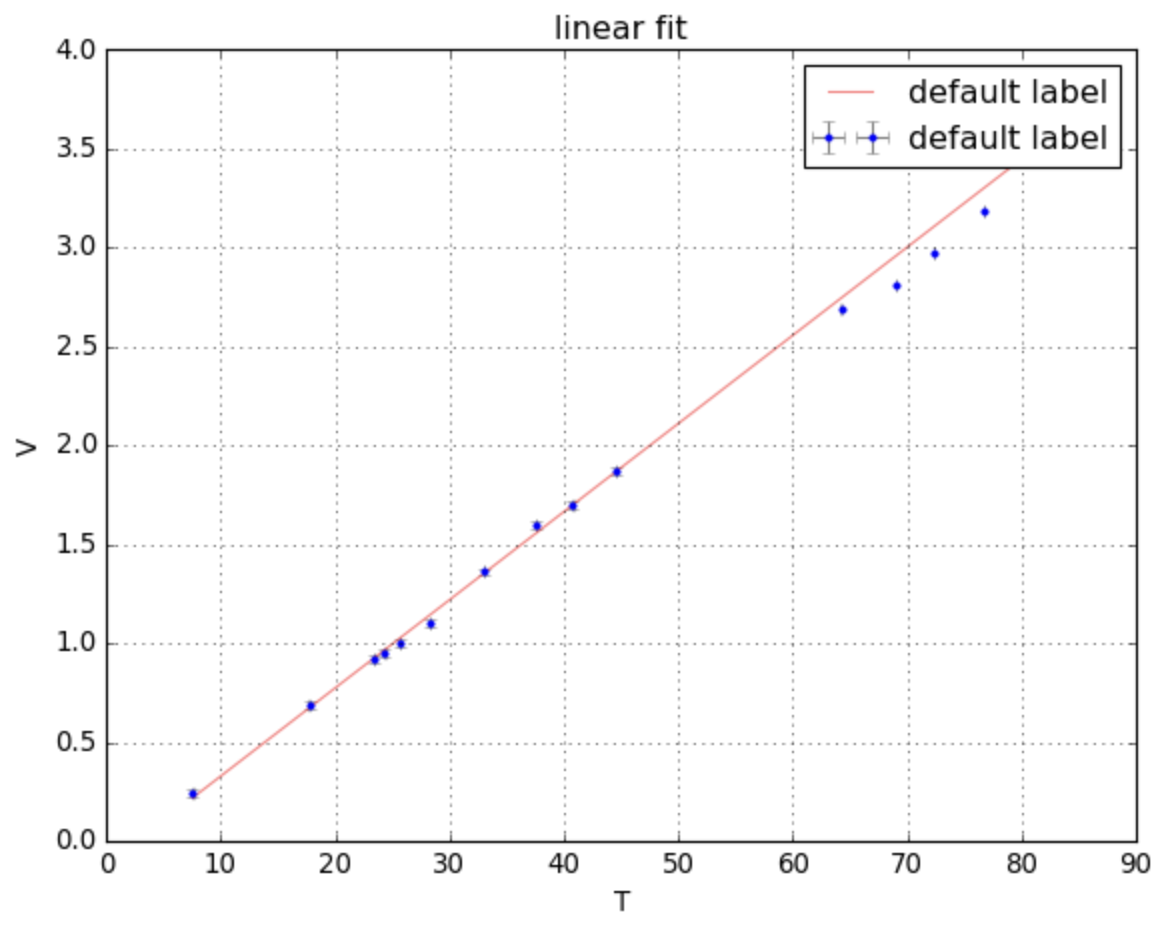
\includegraphics[width=\textwidth]{Part A results/linear fit.png}
      \caption{linear fit}
      \label{fig:partA1}
    \end{subfigure}
    \hfill
    \begin{subfigure}[b]{0.48\textwidth}
      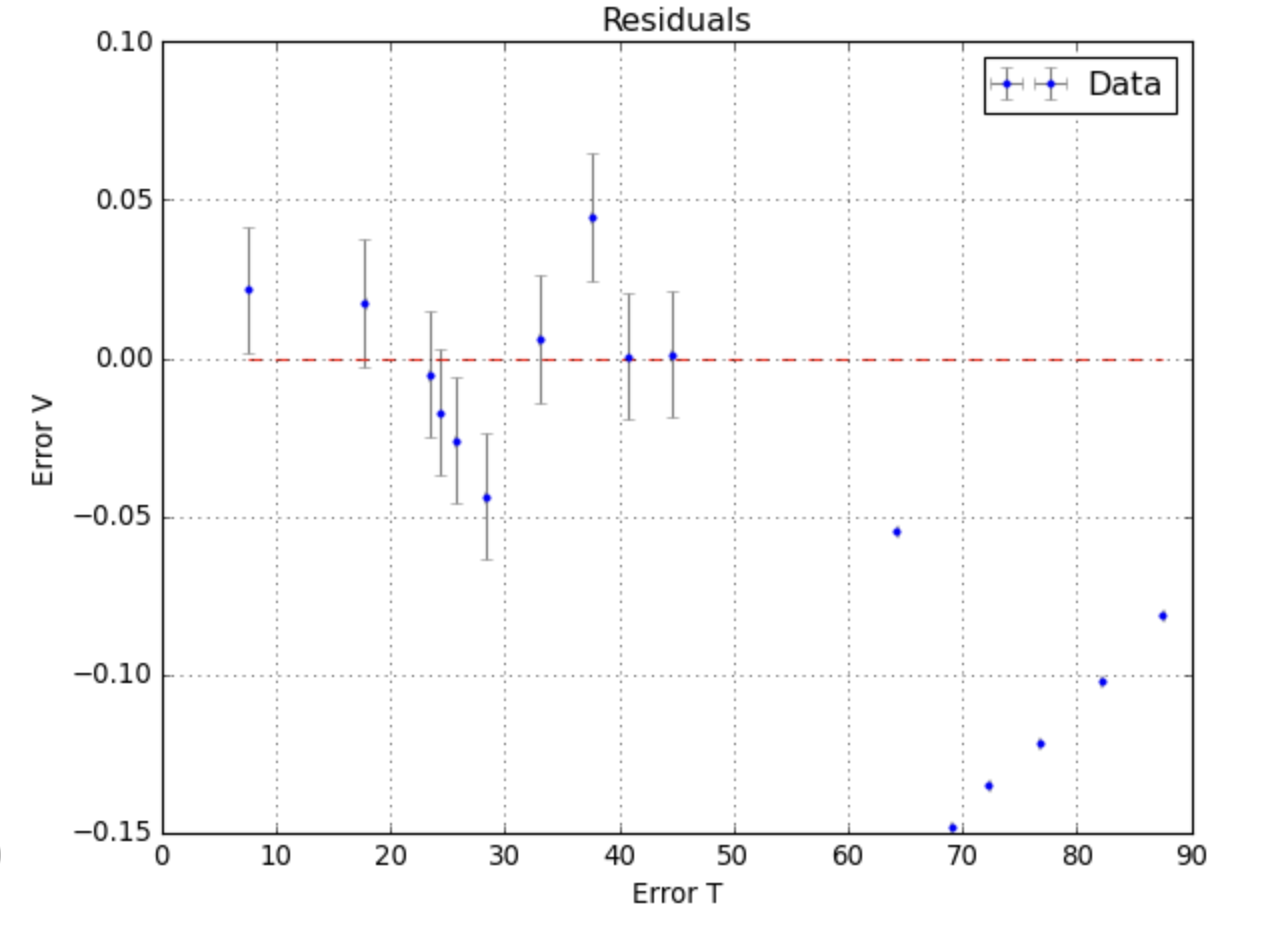
\includegraphics[width=\textwidth]{Part A results/res.png}
      \caption{residual fit}
      \label{fig:partA2}
    \end{subfigure}
    \caption{Part A results}
    \label{fig:partA_results}
  \end{figure}
  
  %------------------------------------------------
  % Table under the figure with four columns
  %------------------------------------------------
  \begin{table}[htbp]
      \centering
      \label{tab:partA_summary}
      \begin{tabular}{@{}cccc@{}}
        \toprule
        $\chi ^2_{reduced}$ & P-probabilty & $a_1$ & $a_0$ \\
        \midrule
        $1.1$ & $0.33$ & $4.32 \cdot 10^{-2} \pm 2.79 \cdot 10^{-4} (0.6\%)$ & $-0.09 \pm 0.01 (13.3\%)$ \\
        \bottomrule
      \end{tabular}
      \caption{Part A results}
    \end{table}
Note that the results were fitted after removing the points arround  $\Delta T = 50$ because they showed a dramatic non linear behavior and a parabolic shape in the residual graph, that hints that it was most likely due to user error.
Taking that into considaraton we see that the ersults agree well with the theoretical model.

Now extracting the values of $V_{room}$ and $V_{nitrogen}$ using interpolation and extrapolation respectively, we get: 
\begin{table}[htbp]
    \centering
    \label{Part A tempreture results}
    \begin{tabular}{@{}cccc@{}}
      \toprule
       $V_{room}$ & $V_{nitrogen}$ \\
      \midrule
      $0.864 \pm 1.727 \cdot 10^{-7} (2 \cdot 10^{-5} \%)$ & $-8.550 \pm 1.529 \cdot 10^{-6} (1.8 \cdot 10^{-5} \%)$ \\
      \bottomrule
    \end{tabular}
    \caption{Tempreture results}
\end{table}
%------------------------------------------------
\pagebreak

And performing the $N_\sigma$ test on both voltages we get:

\begin{table}[htbp]
    \centering
    \label{Part A N-sigma test results}
    \begin{tabular}{@{}cccc@{}}
      \toprule
       $N_{\sigma_{room}} $& $N_{\sigma_{nitrogen}}$ \\
      \midrule
      $0.079$ & $150.079$ \\
      \bottomrule
    \end{tabular}
    \caption{N-sigma test results}

\end{table}
The test concluded that the calculated value of $V_{room}$ is relatively close to the theoretical value. That makes sence looking at the meassurements. 
On the other hand, the test conluded that the calculated value of $V_{nitrogen}$ is far from the theoretiacl value. After taking a closer look it is possible to assume that the relatively small error calculated for the expiremental value is what caused the bad result. 
%------------------------------------------------
% Part B 
%------------------------------------------------

\paragraph{Part B}
After fitting the data to the third order polynomial we get the following results:
%------------------------------------------------

%------------------------------------------------
% Part A results: two subfigures side by side
%------------------------------------------------
\begin{figure}[htbp]
    \centering
    \begin{subfigure}[b]{0.48\textwidth}
      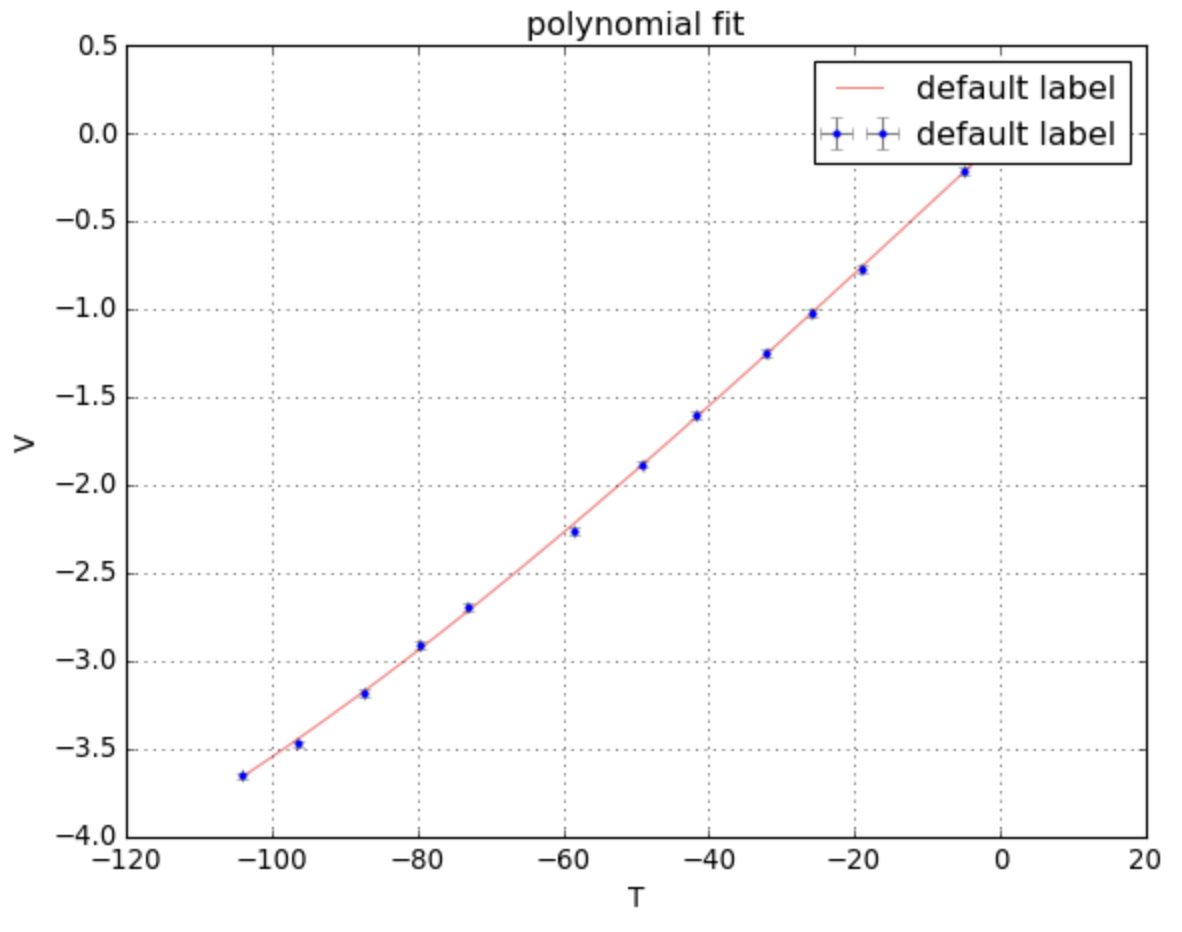
\includegraphics[width=\textwidth]{Part B results/polynomial-fit.png}
      \caption{polynomial fit}
      \label{fig:partB1}
    \end{subfigure}
    \hfill
    \begin{subfigure}[b]{0.48\textwidth}
      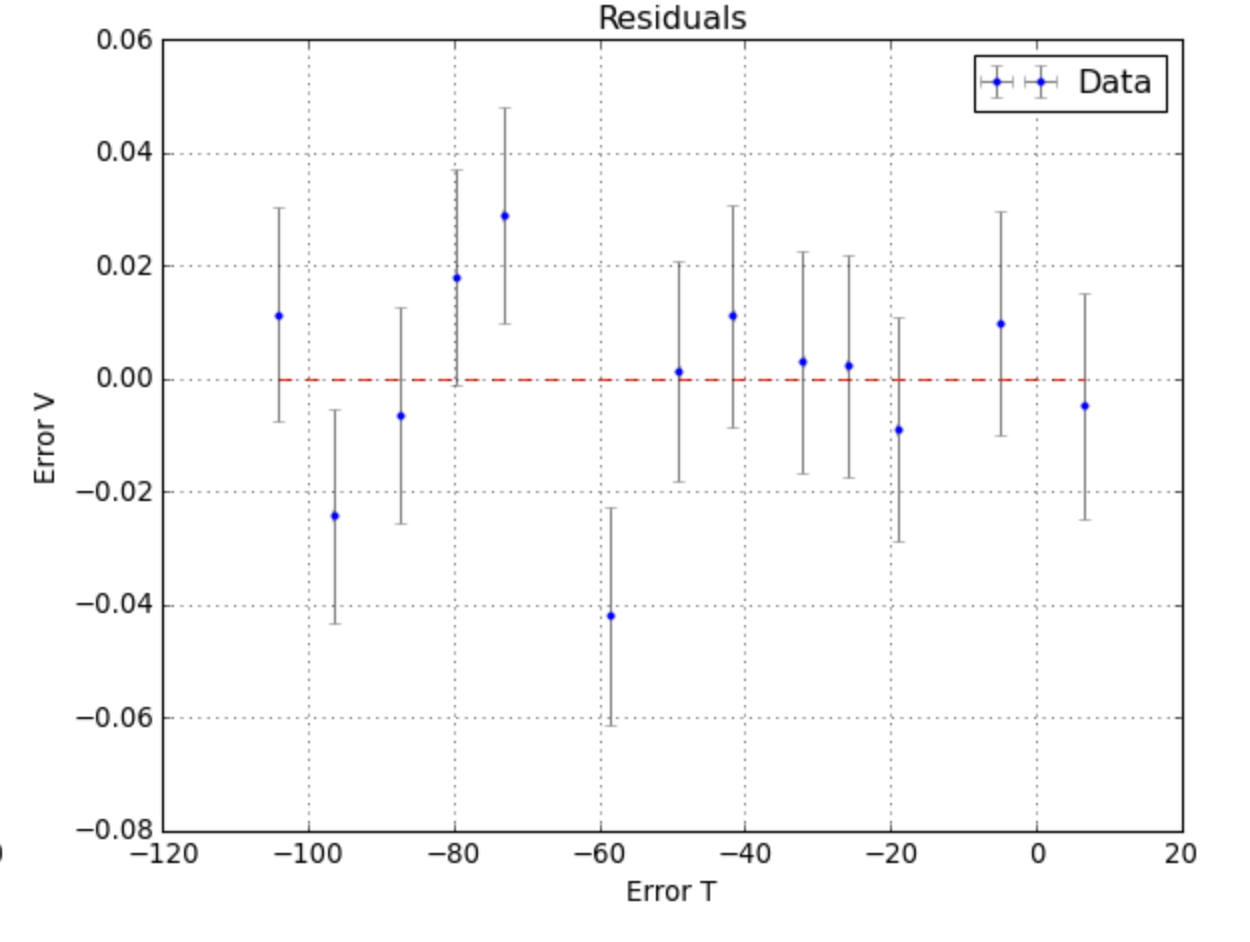
\includegraphics[width=\textwidth]{Part B results/polynomial residual.png}
      \caption{residual fit}
      \label{fig:partB2}
    \end{subfigure}
    \caption{Part B results}
    \label{fig:partB_results}
  \end{figure}
  
  %------------------------------------------------
  % Table under the figure with four columns
  %------------------------------------------------
  \begin{table}[htbp]
    \centering
    \label{tab:partB_summary}
    \resizebox{\textwidth}{!}{%
    \begin{tabular}{@{}cccccc@{}}
      \toprule
      $\chi ^2_{reduced}$ & P-probabilty & $a_0$ & $a_1$ & $a_2$ & $a_3$ \\
      \midrule
      1.197 & 0.2918 & $(-0.02884) \pm (0.01377)(47\%)$ & $(3.8503 \times 10^{-2}) \pm (1.106 \times 10^{-3})(2.8\%)$ & $(-1.969 \times 10^{-6}) \pm (2.7777 \times 10^{-5})(140\%)$ & $(-3.552 \times 10^{-7}) \pm (1.861 \times 10^{-7})(52\%)$ \\
      \bottomrule
    \end{tabular}
    }
    \caption{Part B results}
  \end{table}
  We can see that the $\chi _{reduced}^2$ is close to 1, and the P-probabilty is greater than 0.05, that means that the fit is good and we can use it as an acurate way to measure the voltage for different tempretures. furthermore, $a_0$ is close to 0 taking into consieration its $47.7 \%$ error. 

  \pagebreak
  Now we can intrapolate and extrapolate different values of the voltage for different tempretures.
  \begin{table}[htbp]
    \centering
    \label{Part B tempreture results}
    \begin{tabular}{@{}cccc@{}}
      \toprule
       $V_{room}$ & $V_{nitrogen}$ \\
      \midrule
      $0.8162 \pm 0.0312 (3.8 \%)$ & $-4.976 \pm 1.7687 (35.5 \%)$ \\
      \bottomrule
    \end{tabular}
    \caption{Tempreture results}
\end{table}:

And performing the $N_\sigma$ test on both voltages we get:

\begin{table}[htbp]
    \centering
    \label{Part B N-sigma test results}
    \begin{tabular}{@{}cccc@{}}
      \toprule
       $N_{\sigma_{room}} $& $N_{\sigma_{nitrogen}}$ \\
      \midrule
      $1.716$ & $0.4715$ \\
      \bottomrule
    \end{tabular}
    \caption{N-sigma test results}

\end{table}
Again we get very good results, well within or error range for the value of $V_{room}$. furthermore, the value of $V_{nitrogen}$ is also within the error range of the theoretical value, according to the $N_\sigma$ test.

It is apperent that the polynimial fit described the data better than the linear fit, and that is expected. 

\pagebreak
\section{discussion}

\subsection{Part A}
In Part A, a linear regression over moderate temperature differences yielded a Seebeck coefficient of 
$a_1 = (4.322 \pm 0.028)\times10^{-2}\,\mathrm{mV\,K^{-1}}$ with reduced chi-squared 
$\chi^2_{reduced} = 1.148$ and $P = 0.327$, indicating a statistically satisfactory fit in the restricted range. 
The interpolated room-temperature voltage, $V_{\mathrm{room}} = 0.864 \pm 1.7\times10^{-7}\,\mathrm{V}$, 
agrees within $0.08\,\sigma$ of the theoretical expectation, confirming linearity near ambient conditions. 
However, the extrapolated liquid-nitrogen value deviates by $150\,\sigma$, demonstrating that the linear 
model breaks down at large $\Delta T$ due to the temperature dependence of the Seebeck coefficient and 
nonideal measurement effects.


\subsection{Part B}
In Part B, a third-order polynomial fit captures the full temperature span with 
$\chi^2_{reduced} = 1.197$ and $P = 0.292$, showing that higher-order terms are necessary to model the 
observed nonlinearity. The extracted voltages, $V_{\mathrm{room}} = 0.816 \pm 0.031\,\mathrm{V}$ and 
$V_{\mathrm{nitrogen}} = -4.976 \pm 1.769\,\mathrm{V}$, both fall within $3\,\sigma$ of their theoretical 
values, validating the polynomial calibration. This improved model provides an accurate calibration curve, highlighting the limitations of simple linear approximations 
across wide temperature ranges.

\pagebreak
\appendix
\setcounter{figure}{0}
\setcounter{table}{0}
\section{Appendix: Figures}

\begin{figure}[H]
    \centering
    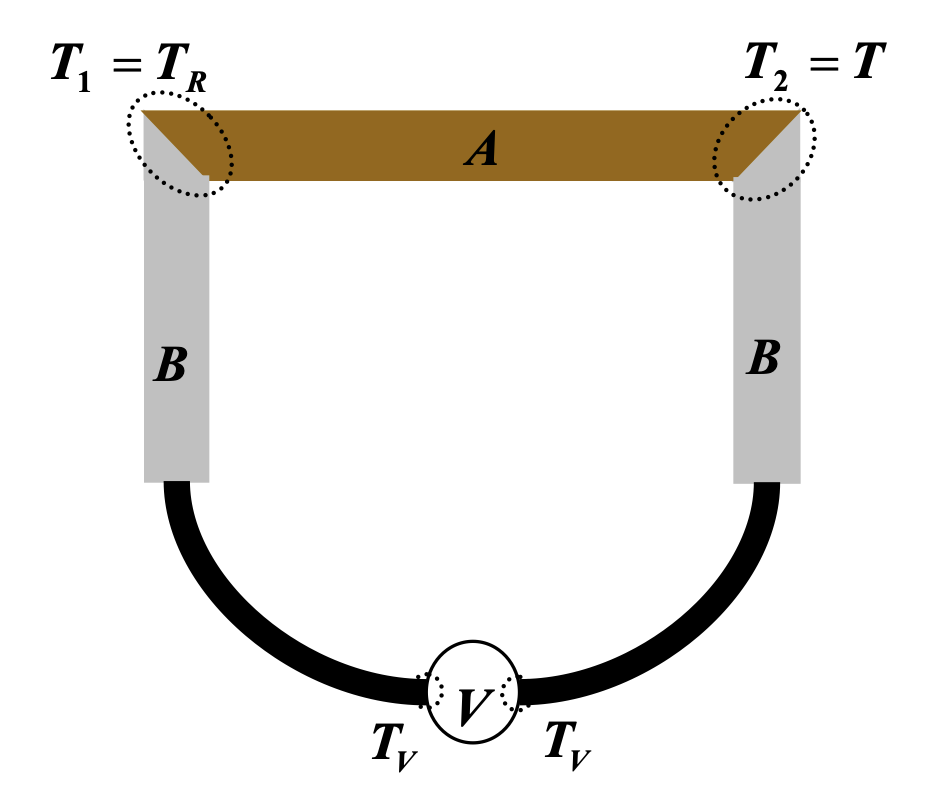
\includegraphics[width=0.5\textwidth]{general IMG/Kthermo.png}
    \caption{Thermocouple}
    \label{fig:thermocouple}
\end{figure}

\begin{figure}[H]
    \centering
    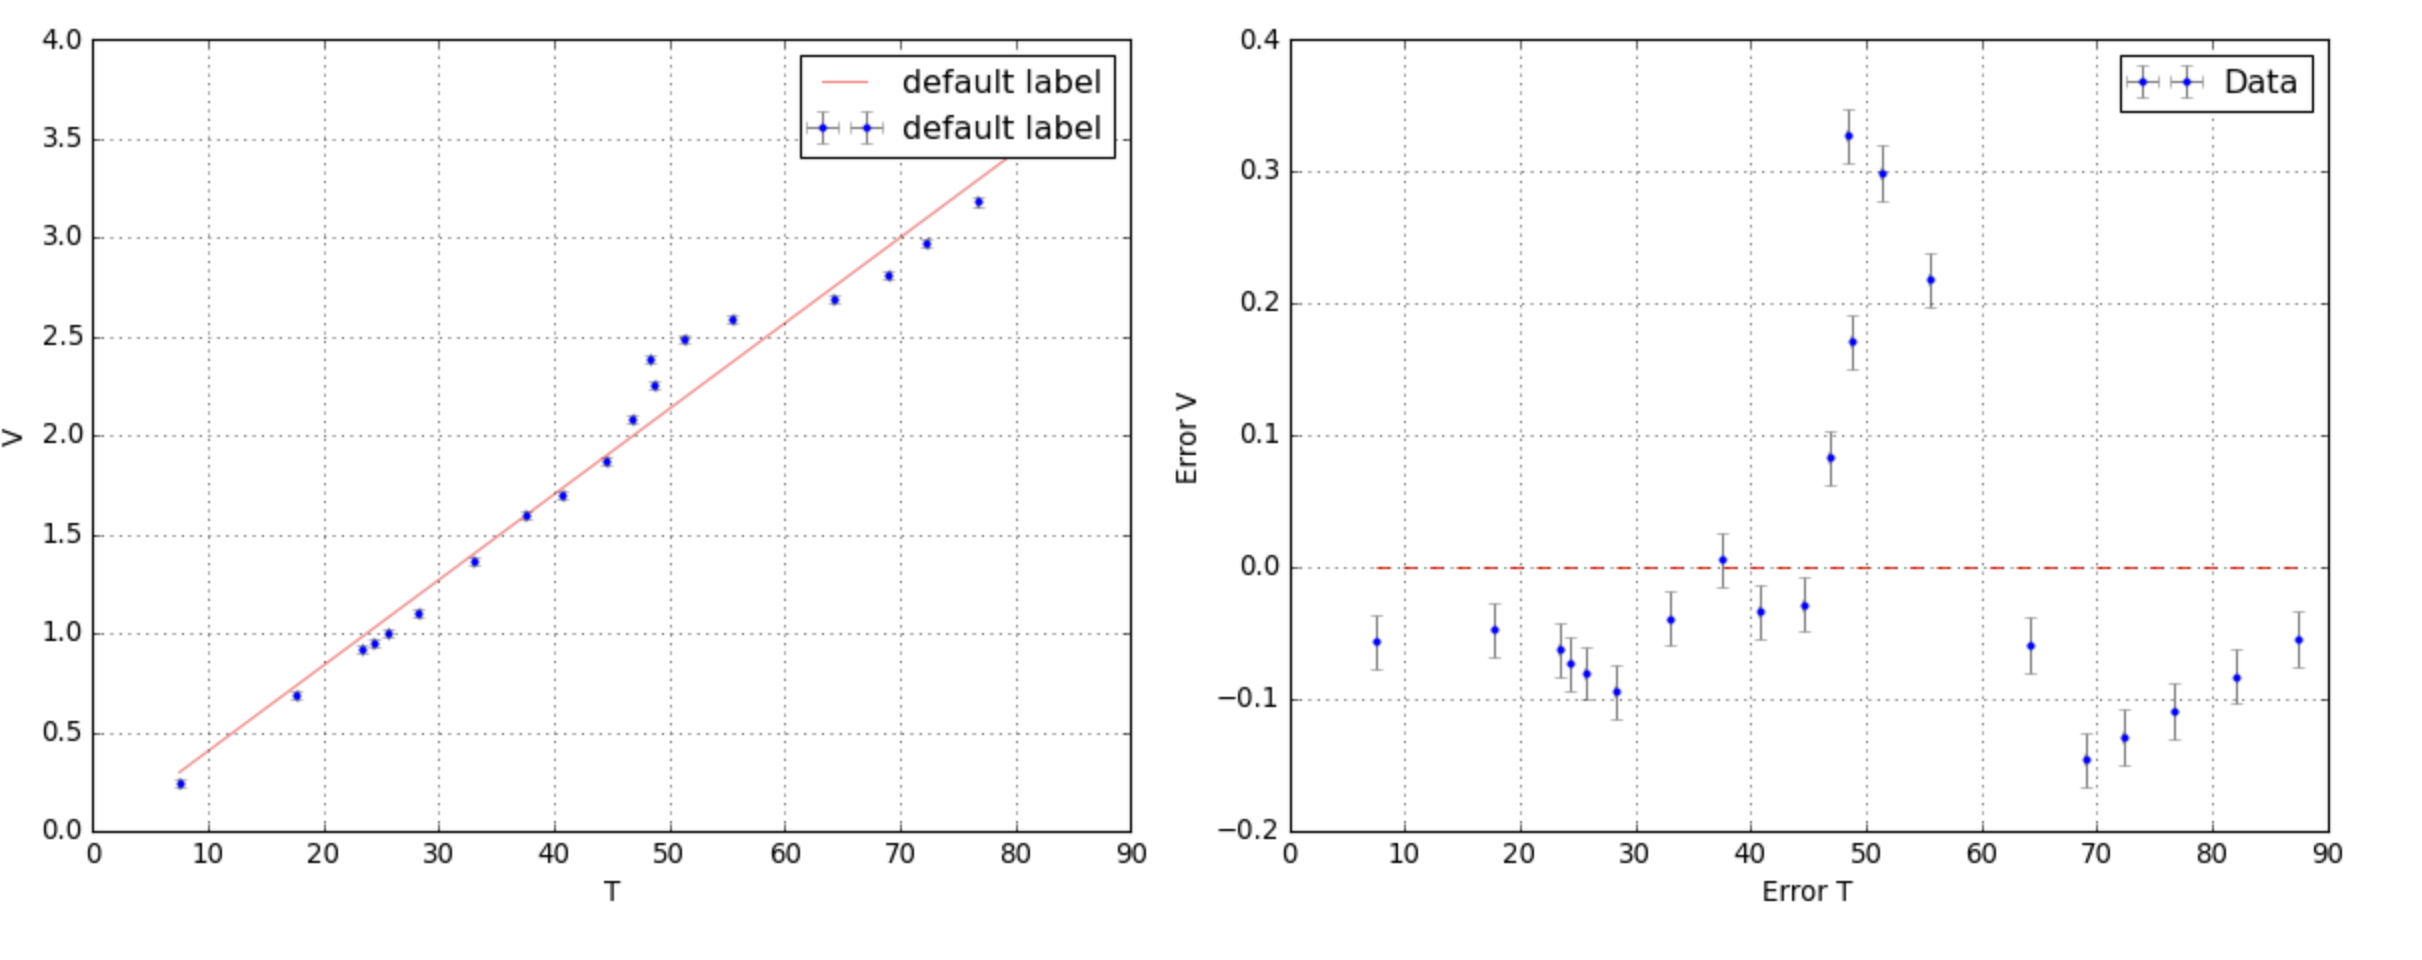
\includegraphics[width=0.7\textwidth]{Part A results/full set linear fit.png}
    \caption{linear fit  and residual of the unmodifyed set, part A}
    \label{fig:appendix_partA_full_set_fit}
\end{figure}


\begin{figure}[H]
    \centering
    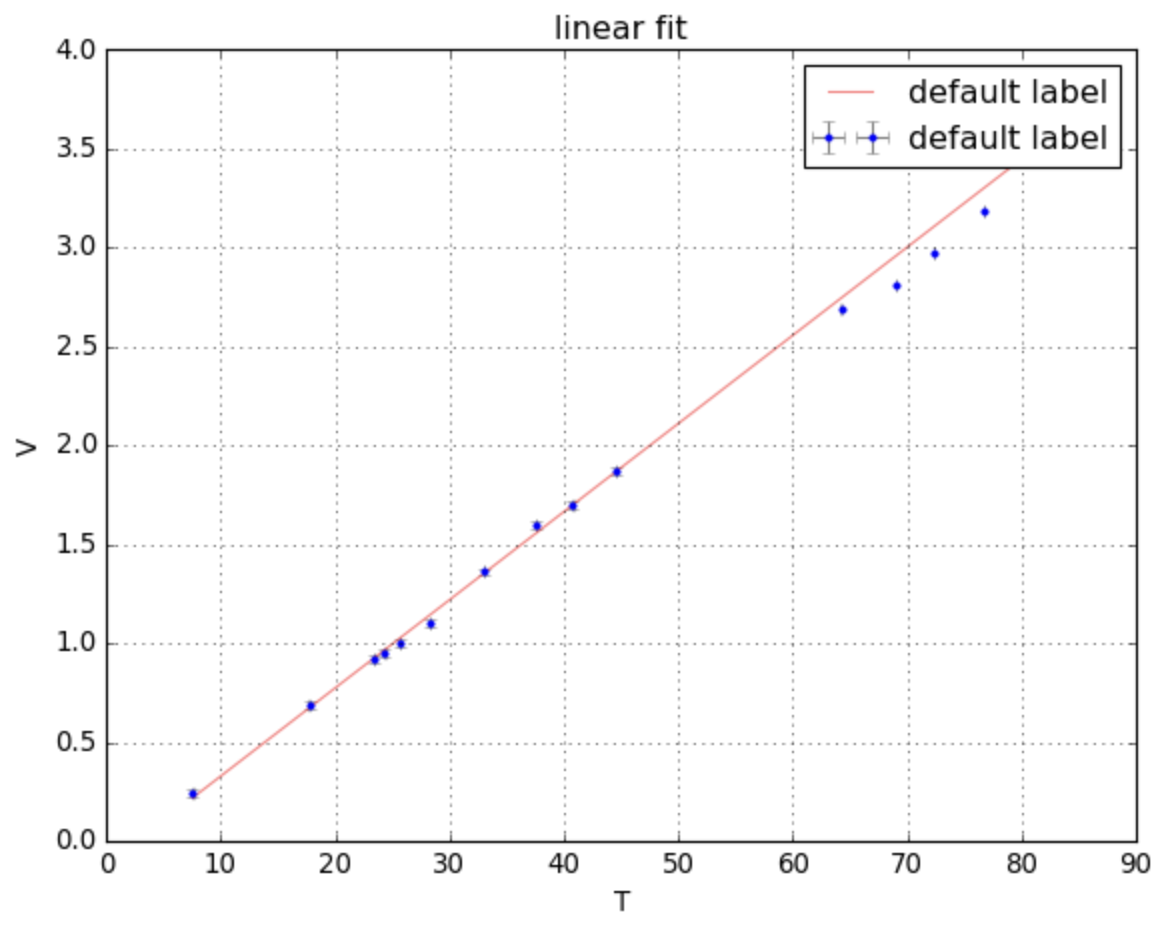
\includegraphics[width=0.7\textwidth]{Part A results/linear fit.png}
    \caption{Linear fit for Part A}
    \label{fig:appendix_partA_linear_fit}
\end{figure}

\begin{figure}[H]
    \centering
    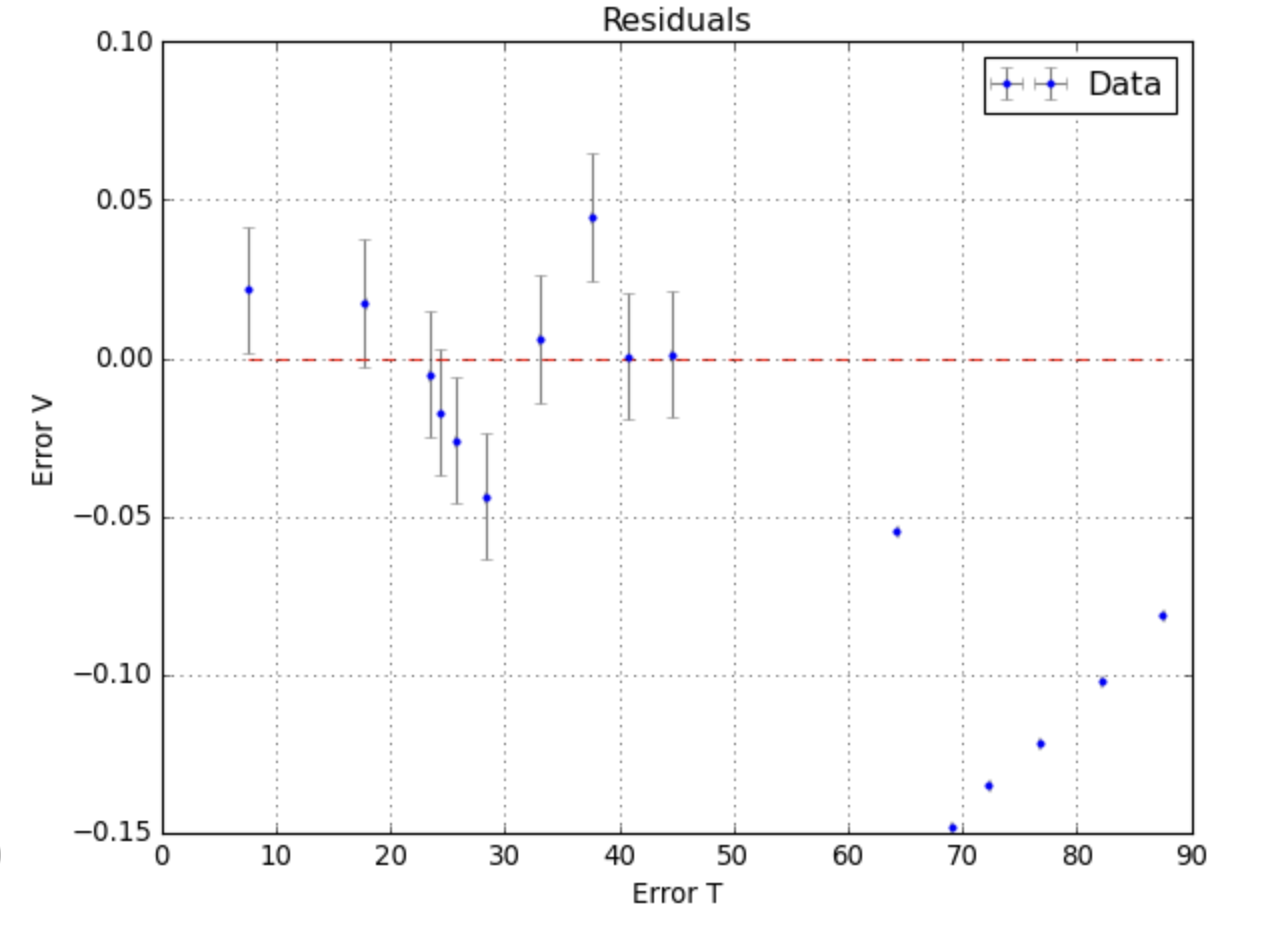
\includegraphics[width=0.7\textwidth]{Part A results/res.png}
    \caption{Residual fit for Part A}
    \label{fig:appendix_partA_residual_fit}
\end{figure}

\begin{figure}[H]
    \centering
    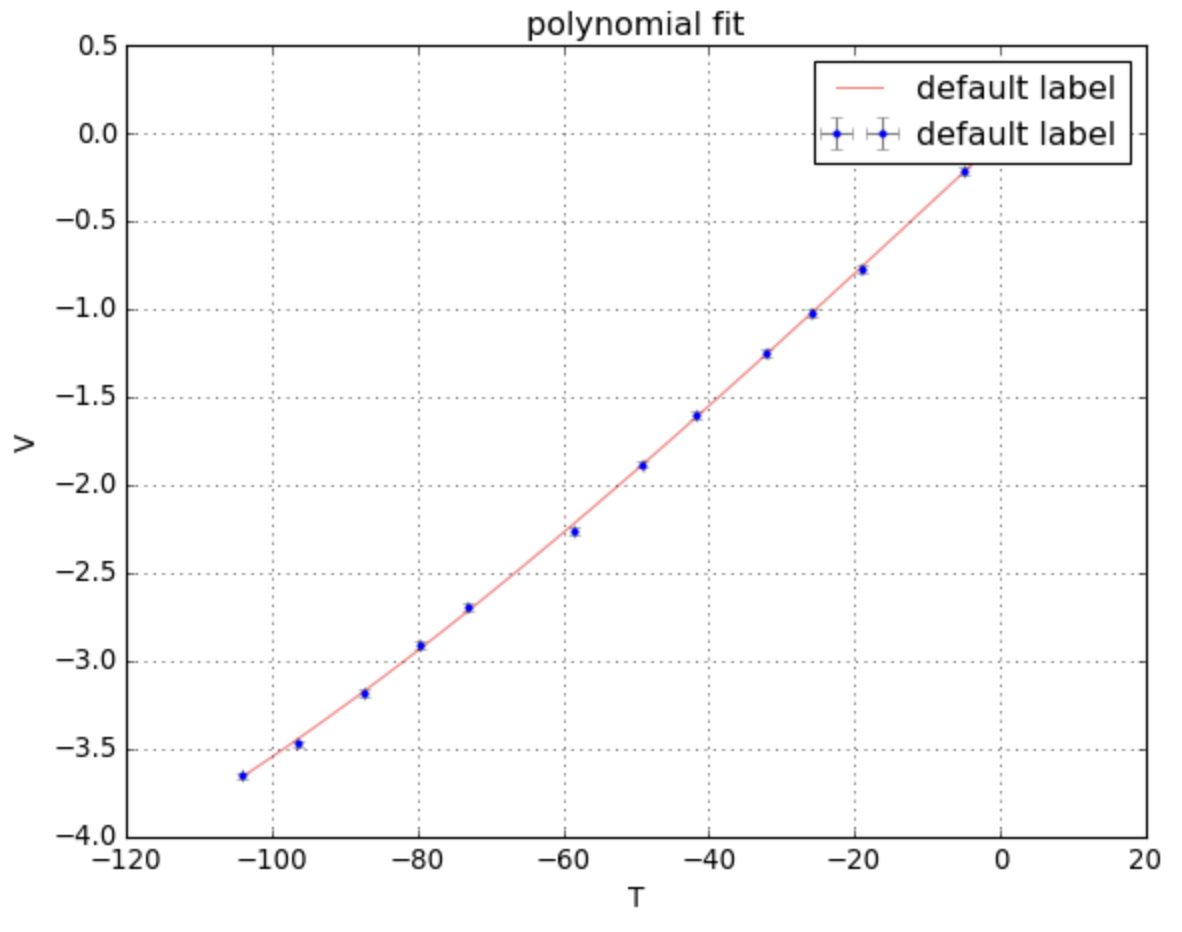
\includegraphics[width=0.7\textwidth]{Part B results/polynomial-fit.png}
    \caption{Polynomial fit for Part B}
    \label{fig:appendix_partB_polynomial_fit}
\end{figure}

\begin{figure}[H]
    \centering
    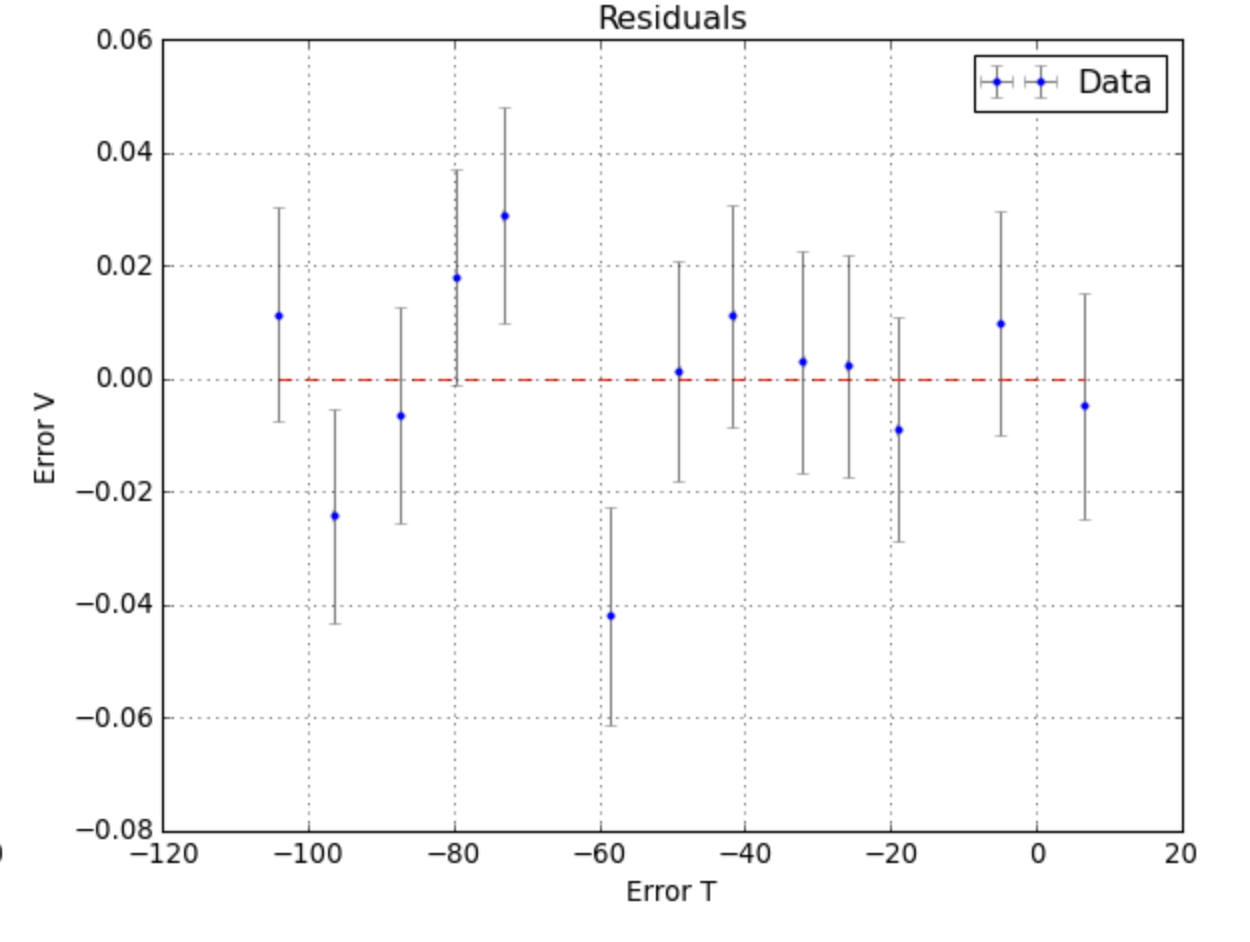
\includegraphics[width=0.7\textwidth]{Part B results/polynomial residual.png}
    \caption{Residual fit for Part B}
    \label{fig:appendix_partB_residual_fit}
\end{figure}

\pagebreak

\section{Appendix: tables}

\begin{table}[H]
\centering
\begin{tabular}{|l|l|l|}
\hline
$T[C]$ & $V[mV]$  & $\Delta V$     \\
82.108   & 3.44       & 0.021032 \\ \hline
76.708   & 3.18       & 0.020954 \\ \hline
72.3     & 2.97       & 0.020891 \\ \hline
69.008   & 2.81       & 0.020843 \\ \hline
64.217   & 2.69       & 0.020807 \\ \hline
55.51    & 2.59       & 0.020777 \\ \hline
51.33    & 2.49       & 0.020747 \\ \hline
48.36    & 2.39       & 0.020717 \\ \hline
48.74    & 2.25       & 0.020675 \\ \hline
46.84    & 2.08       & 0.020624 \\ \hline
44.56    & 1.87       & 0.020561 \\ \hline
40.76    & 1.7        & 0.02051  \\ \hline
37.533   & 1.6        & 0.02048  \\ \hline
33.013   & 1.36       & 0.020408 \\ \hline
28.287   & 1.1        & 0.02033  \\ \hline
25.65    & 1          & 0.0203   \\ \hline
24.332   & 0.95       & 0.020285 \\ \hline
23.39    & 0.92       & 0.020276 \\ \hline
17.72    & 0.69       & 0.020207 \\ \hline
7.533    & 0.24       & 0.020072 \\ \hline

\end{tabular}
\caption{first set of measurments}
\end{table}

\begin{table}[H]
\centering
\begin{tabular}{|l|l|}
\hline
\textbf{T} & \textbf{V}  \\ \hline
\textbf{6.592}    & \textbf{0.22}       \\ \hline
\textbf{-4.96}    & \textbf{-0.21}      \\ \hline
\textbf{-19.067}  & \textbf{-0.77}      \\ \hline
\textbf{-25.93}   & \textbf{-1.02}      \\ \hline
\textbf{-32.045}  & \textbf{-1.25}      \\ \hline
\textbf{-41.675}  & \textbf{-1.6}       \\ \hline
\textbf{-49.079}  & \textbf{-1.88}      \\ \hline
\textbf{-58.533}  & \textbf{-2.26}      \\ \hline
\textbf{-73.217}  & \textbf{-2.69}      \\ \hline
\textbf{-79.633}  & \textbf{-2.91}      \\ \hline
\textbf{-87.457}  & \textbf{-3.18}      \\ \hline
\textbf{-96.58}   & \textbf{-3.47}      \\ \hline
\textbf{-104.24}  & \textbf{-3.65}      \\ \hline
\end{tabular}

\caption{Second set of meassurments}
\end{table}

\end{document}
